\documentclass[a4paper,11pt,exos]{nsi} % COMPILE WITH DRAFT
\usepackage{hyperref}

\pagestyle{empty}
\begin{document}


\classe{\premiere spe}
\titre{Suites arithmétiques et géométriques}
\maketitle
\section*{Partie B}


\exo{ : Compléter les suites logiques}
\renewcommand{\arraystretch}{1.6}
\begin{tabular}{|c|c|c|c|c|c|c|c|c|c|}
	\hline
	\rowcolor{UGLiOrange}Rang & \hspace{0.5cm}0\hspace{0.5cm} & \hspace{0.5cm}1\hspace{0.5cm} & \hspace{0.5cm}2\hspace{0.5cm} & \hspace{0.5cm}3\hspace{0.5cm} & \hspace{0.5cm}4\hspace{0.5cm} & \hspace{0.5cm}5\hspace{0.5cm} & \hspace{0.5cm}6\hspace{0.5cm} & \hspace{0.5cm}7\hspace{0.5cm} & \hspace{0.5cm}8\hspace{0.5cm}  \\
	\hline
	\cellcolor{UGLiOrange}Suite 1 : & $1$ & $3$ & $5$ & $7$ & $9$ & & & & \\
	\hline
	\cellcolor{UGLiOrange}Suite 2 : & $81$ & $27$ & $9$ & $3$ & $1$ & & & & \\
	\hline
	\cellcolor{UGLiOrange}Suite 3 : & $15$ & $10$ & $5$ & $0$ & $-5$ & & & & \\
	\hline
	\cellcolor{UGLiOrange}Suite 4 : & $8$ & $-4$ & $2$ & $-1$ & $\dfrac{1}{2}$ & & & & \\
	\hline
	\cellcolor{UGLiOrange}Suite 5 : & $1$ & $5$ & $13$ & $29$ & $61$ & & & & \\
	\hline
\end{tabular}


\begin{definition}[]
	Une suite $(u_n)$ est dite \textbf{arithmétique} s'il existe un réel $r$ tel que pour tout entier $n$ on a  $u_{n+1}=u_n+r$.\\
	Cette expression est appelée formule de récurrence.\\
	Le nombre $r$ est appelé \textbf{raison} de la suite $(u_n)$.
\end{definition}

\begin{definition}[]
	Une suite $(u_n)$ est dite \textbf{géométrique} s'il existe un réel $q$ tel que pour tout entier $n$ on a  $u_{n+1}=q\times u_n$.\\
	Cette expression est appelée formule de récurrence.\\
	Le nombre $q$ est appelé \textbf{raison} de la suite $(u_n)$.
\end{definition}



%\newpage
\exo{ : Compléter lorsque la suite est soit arithmétique, soit géométrique}
\begin{tabular}{|c|p{3.5cm}|p{3.5cm}|c|c|c|}
	\hline
	 & Relation de récurrence de la suite & \centering Nature & $u_0$ & $u_1$ & $u_{10}$ \\
	 \hline
	 Suite 1 & & & \hspace{1.5cm} & \hspace{1.5cm} & \hspace{1.5cm} \\
	 \hline
	 Suite 2 & & & \hspace{.9cm} & \hspace{.9cm} & \hspace{.9cm} \\
	 \hline
	 Suite 3 & & & \hspace{.9cm} & \hspace{.9cm} & \hspace{.9cm} \\
	 \hline
	 Suite 4 & & & \hspace{.9cm} & \hspace{.9cm} & \hspace{.9cm} \\
	 \hline
	 Suite 5 & & & \hspace{.9cm} & \hspace{.9cm} & \hspace{.9cm} \\
	 \hline
\end{tabular}



\begin{encadrecolore}{Tutoriel}{UGLiOrange}
	Pour représenter la suite $(u_n)$ définie $u_0=0$ et par la relation de récurrence $u_{n+1}=0,4u_n+6$ :\\
	
	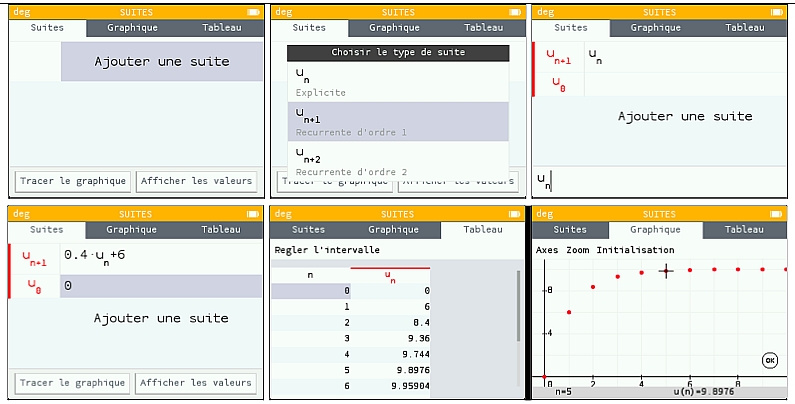
\includegraphics[width=16.5cm]{calculatrice}\\[.5em]
	\begin{minipage}{2cm}
		
\includegraphics[width=1.5cm]{qr_code}
	\end{minipage}
	\begin{minipage}{12cm}
		\textbf{Tutoriel vidéo :}\\
		\href{https://www.numworks.com/fr/professeurs/tutoriels/suites/}{https://www.numworks.com/fr/professeurs/tutoriels/suites/}
	\end{minipage}
	
\end{encadrecolore}



\exo{ Représenter graphiquement à la calculatrice les termes de suites 1, 2, 3 et 4.}
Que remarque-t-on pour les suites 1 et 3 ?\\[.5em]
\carreauxseyes{16.8}{1.6}\\

Quel semble être le sens de variation des suites 1 et 3 ? Pourquoi ?\\[.5em]
\carreauxseyes{16.8}{1.6}
\end{document}